% !TeX spellcheck = es_ES
% Chapter 1

%\chapter{Chapter Title Here} % Main chapter title
%
%\label{Chapter1} % For referencing the chapter elsewhere, use \ref{Chapter1} 

%----------------------------------------------------------------------------------------

% Define some commands to keep the formatting separated from the content 
%\newcommand{\keyword}[1]{\textit{#1}}
%\newcommand{\tabhead}[1]{\textbf{#1}}
%\newcommand{\code}[1]{\texttt{#1}}
%\newcommand{\file}[1]{\texttt{\bfseries#1}}
%\newcommand{\option}[1]{\texttt{\itshape#1}}

%----------------------------------------------------------------------------------------

\chapter{Instalación del calorímetro}
	El calorímetro originalmente era usado en la Universidad Sueca de Ciencias Agrícolas, en donde la red eléctrica es de 230 VAC. En Colombia se usan 110 VAC, razón por la cual una parte importante de la instalación del calorímetro consistió en configurar las entradas de voltaje del equipo para su operación en el país. Para esto fue necesario cambiar 2 fusibles por unos con capacidad para el doble de corriente, pues en los circuitos eléctricos con transformadores que permiten ajustar el voltaje de entrada, se tiene que conservar la potencia, la cual está dada por el producto de corriente y voltaje. Los fusibles se encuentran en el panel inferior derecho del calorímetro (\autoref{fig: fuseBox}), y en la parte trasera, los nuevos fusibles tienen valores de corriente de 4 A y 6 A, correspondientemente. Junto con este cambio fue necesario modificar las perillas selectoras de voltaje, una de las cuales se encuentra en el mismo panel del primer fusible (\autoref{fig: fuseBox}) mientras que el otro está en la parte trasera del módulo de control de la temperatura (\autoref{fig: decadeResistors}), el valor seleccionado es de 115 VAC.
	\begin{figure}[h]
		\centering
		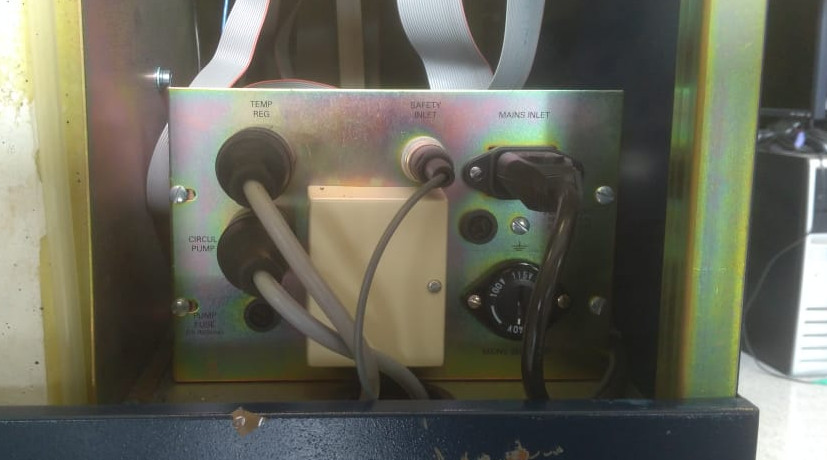
\includegraphics[width=0.7\linewidth]{Figures/fusepanel}
		\caption{Panel de selección de voltaje del calorímetro.}
		\label{fig: fuseBox}
	\end{figure}

	Posteriormente, uno de los cilindros de medición fue identificado en una de las cajas, se fijó al baño interno, y se llevaron a cabo las conexiones eléctricas con el módulo de amplificación como se muestra a continuación. 
	\begin{figure}[h]
		\centering
		\begin{tabular}{cccc}
			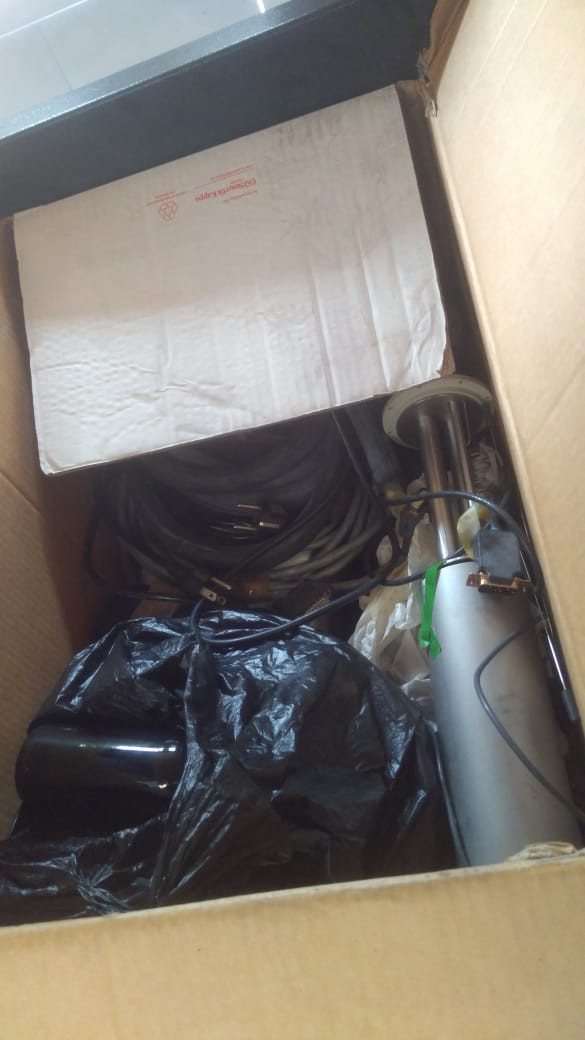
\includegraphics[width=0.24\linewidth]{Figures/process/box1} & 
			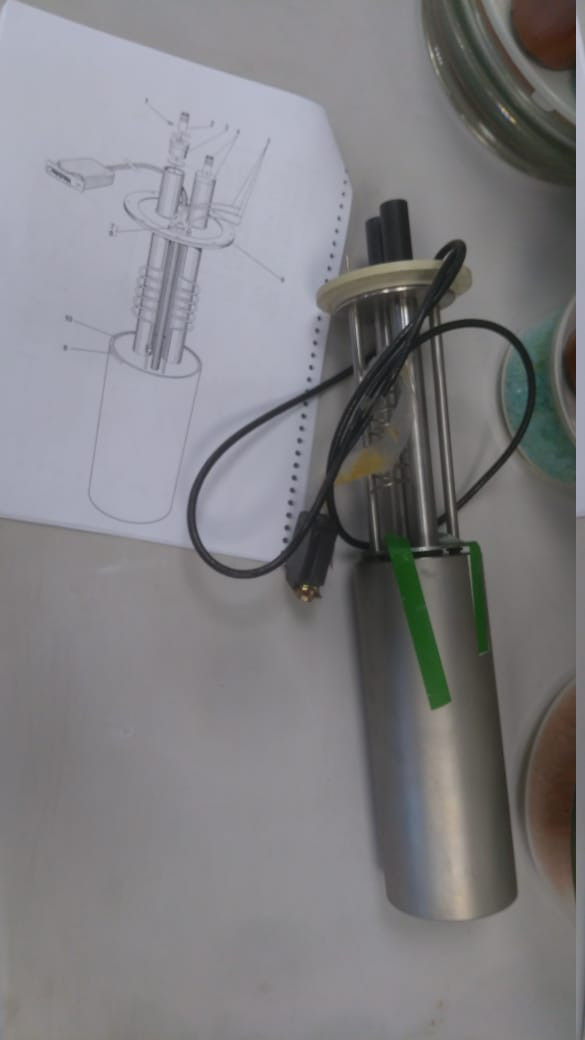
\includegraphics[width=0.24\linewidth]{Figures/process/holder} &
			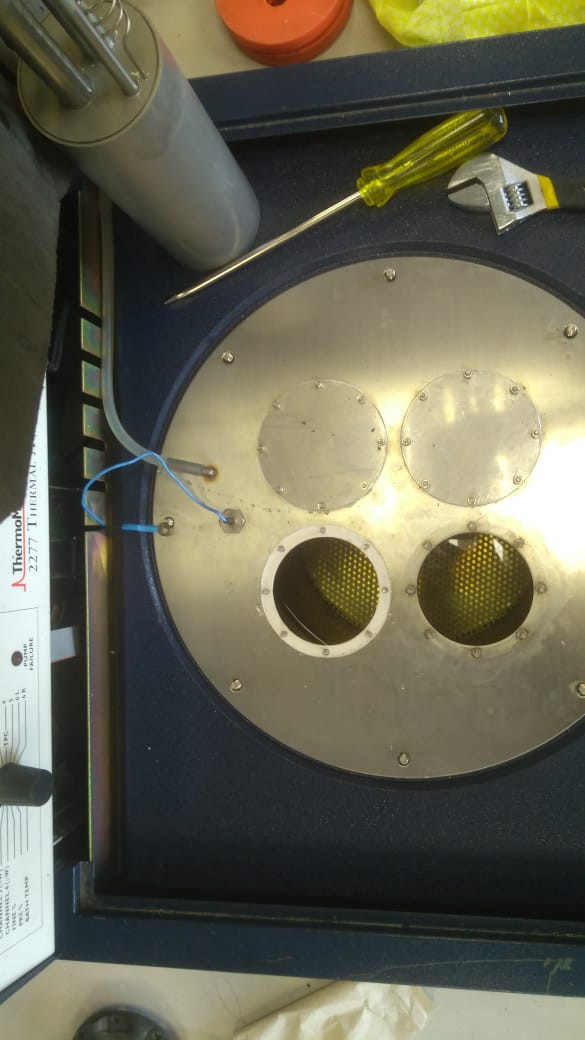
\includegraphics[width=0.24\linewidth]{Figures/process/p1} & 
			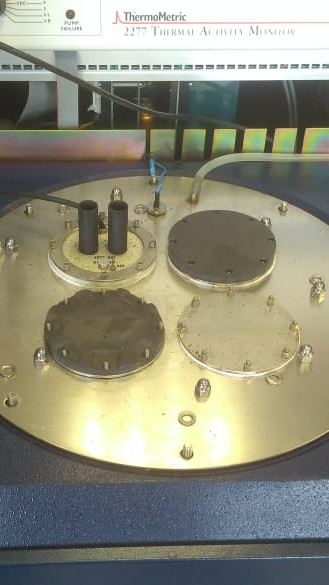
\includegraphics[width=0.24\linewidth]{Figures/process/p2} \\
			& 
			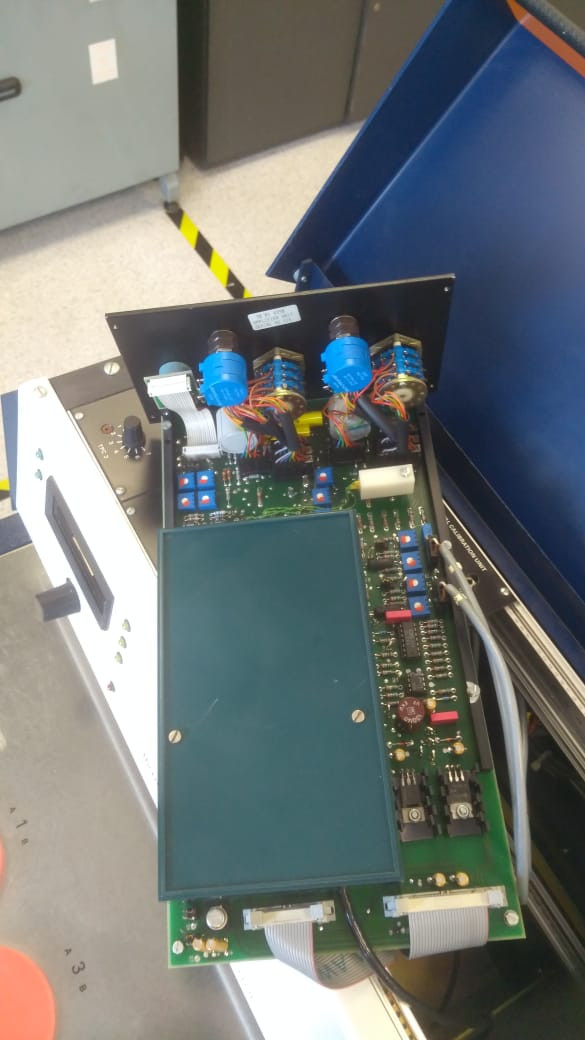
\includegraphics[width=0.24\linewidth]{Figures/process/p3} &
			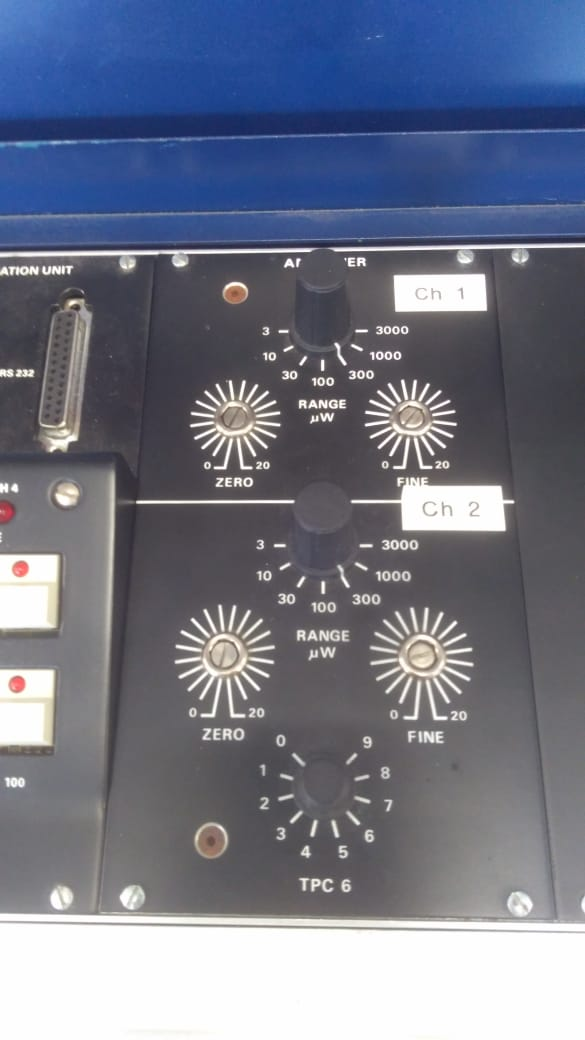
\includegraphics[width=0.24\linewidth]{Figures/process/p4} &
		\end{tabular}
		\caption{Proceso de instalación de un cilindro de medición.}
		\label{fig: instalationMultiple}
	\end{figure}

	
	
	\section{Software de control}
	\subsection{Configuración del equipo}
	\subsection{Creación de un método experimental}
	\subsection{Control del experimento}
	\subsection{Configuración de la gráfica}
	\subsection{Lectura de resultados}
	\section{Efecto del agitador en las lecturas}
	Para comprobar el efecto del agitador en la potencia registrada por el equipo se llevaron a cabo 6 ciclos de conexión desconexión con 15 minutos entre cada perturbación al sistema, horas después de haber realizado una calibración estática. Las diferencias de potencia generadas entre cada conexión (izquierda) y desconexión (derecha) se muestran en la \autoref{tb: connection}, y también en la \autoref{fig: connection}, donde se observan como aumentos y descensos súbitos en la potencia registrada.
	\begin{table}[h]
		\centering
		\caption{Efectos inmediatos de conectar y desconectar el agitador.}
		\begin{tabular}{cc|l|cc|l}
			\hline
			\textbf{Antes ($\mu$W)} & \textbf{Después ($\mu$W)} &  $\Delta$ ($\mu$W) &  \textbf{Antes ($\mu$W)} & \textbf{Después ($\mu$W)} &  $\Delta$ ($\mu$W) \\
			\hline
			-7,58 &  -5.5 & 2,08 & -5,84 & -7,78 & -1,94 \\
			-6,12 & -3.78 & 2,34 & -5,12 & -7,04 & -1,92 \\
			-5,04 & -2.76 & 2,28 & -4,17 & -6,48 & -2,31 \\
			-5,43 & -3.21 & 2,22 & -5,22 & -7,31 & -2,09 \\
			-6,65 & -4.72 & 1,93 & -6,71 & -8,54 & -1,83 \\
			-7,75 & -5.84 & 1,91 & -8,35 & -9,93 & -1,58 \\
			\hline
			 & \textbf{promedio} ($\mu$W) & 2,1 $\pm$ 0,2 & & & -1,9 $\pm$ 0,2 \\
			\hline
		\end{tabular}
		\label{tb: connection}
	\end{table}

	A partir de los datos de la \autoref{tb: connection} fue posible establecer que el efecto de prender y apagar el agitador es de aproximadamente 2 $\mu$W, siendo un aumento en el caso de conexión y una disminución al desconectarlo. Lo anterior tiene sentido, pues el agitador realiza trabajo sobre la solución, por lo cual al tener un sistema isotérmico la energía se transmite en forma de calor, y de forma diferencial será registrado como un aumento de potencia en el calorímetro. La \autoref{fig: connection} por su lado, muestra que este efecto es local en el tiempo y que el sistema tiende a equilibrarse nuevamente al valor de la línea base. Esto se infiere pues el sistema luego de registrar el aumento súbito experimenta una disminución de la potencia lenta, lo contrario ocurre con la desconexión, por lo cual el sistema tiende a retomar el equilibrio dado por la curva naranja, la cual se obtiene realizando mínimos cuadrados con los datos sobre un polinomio de grado 2.
	
	\begin{figure}[h]
		\centering
		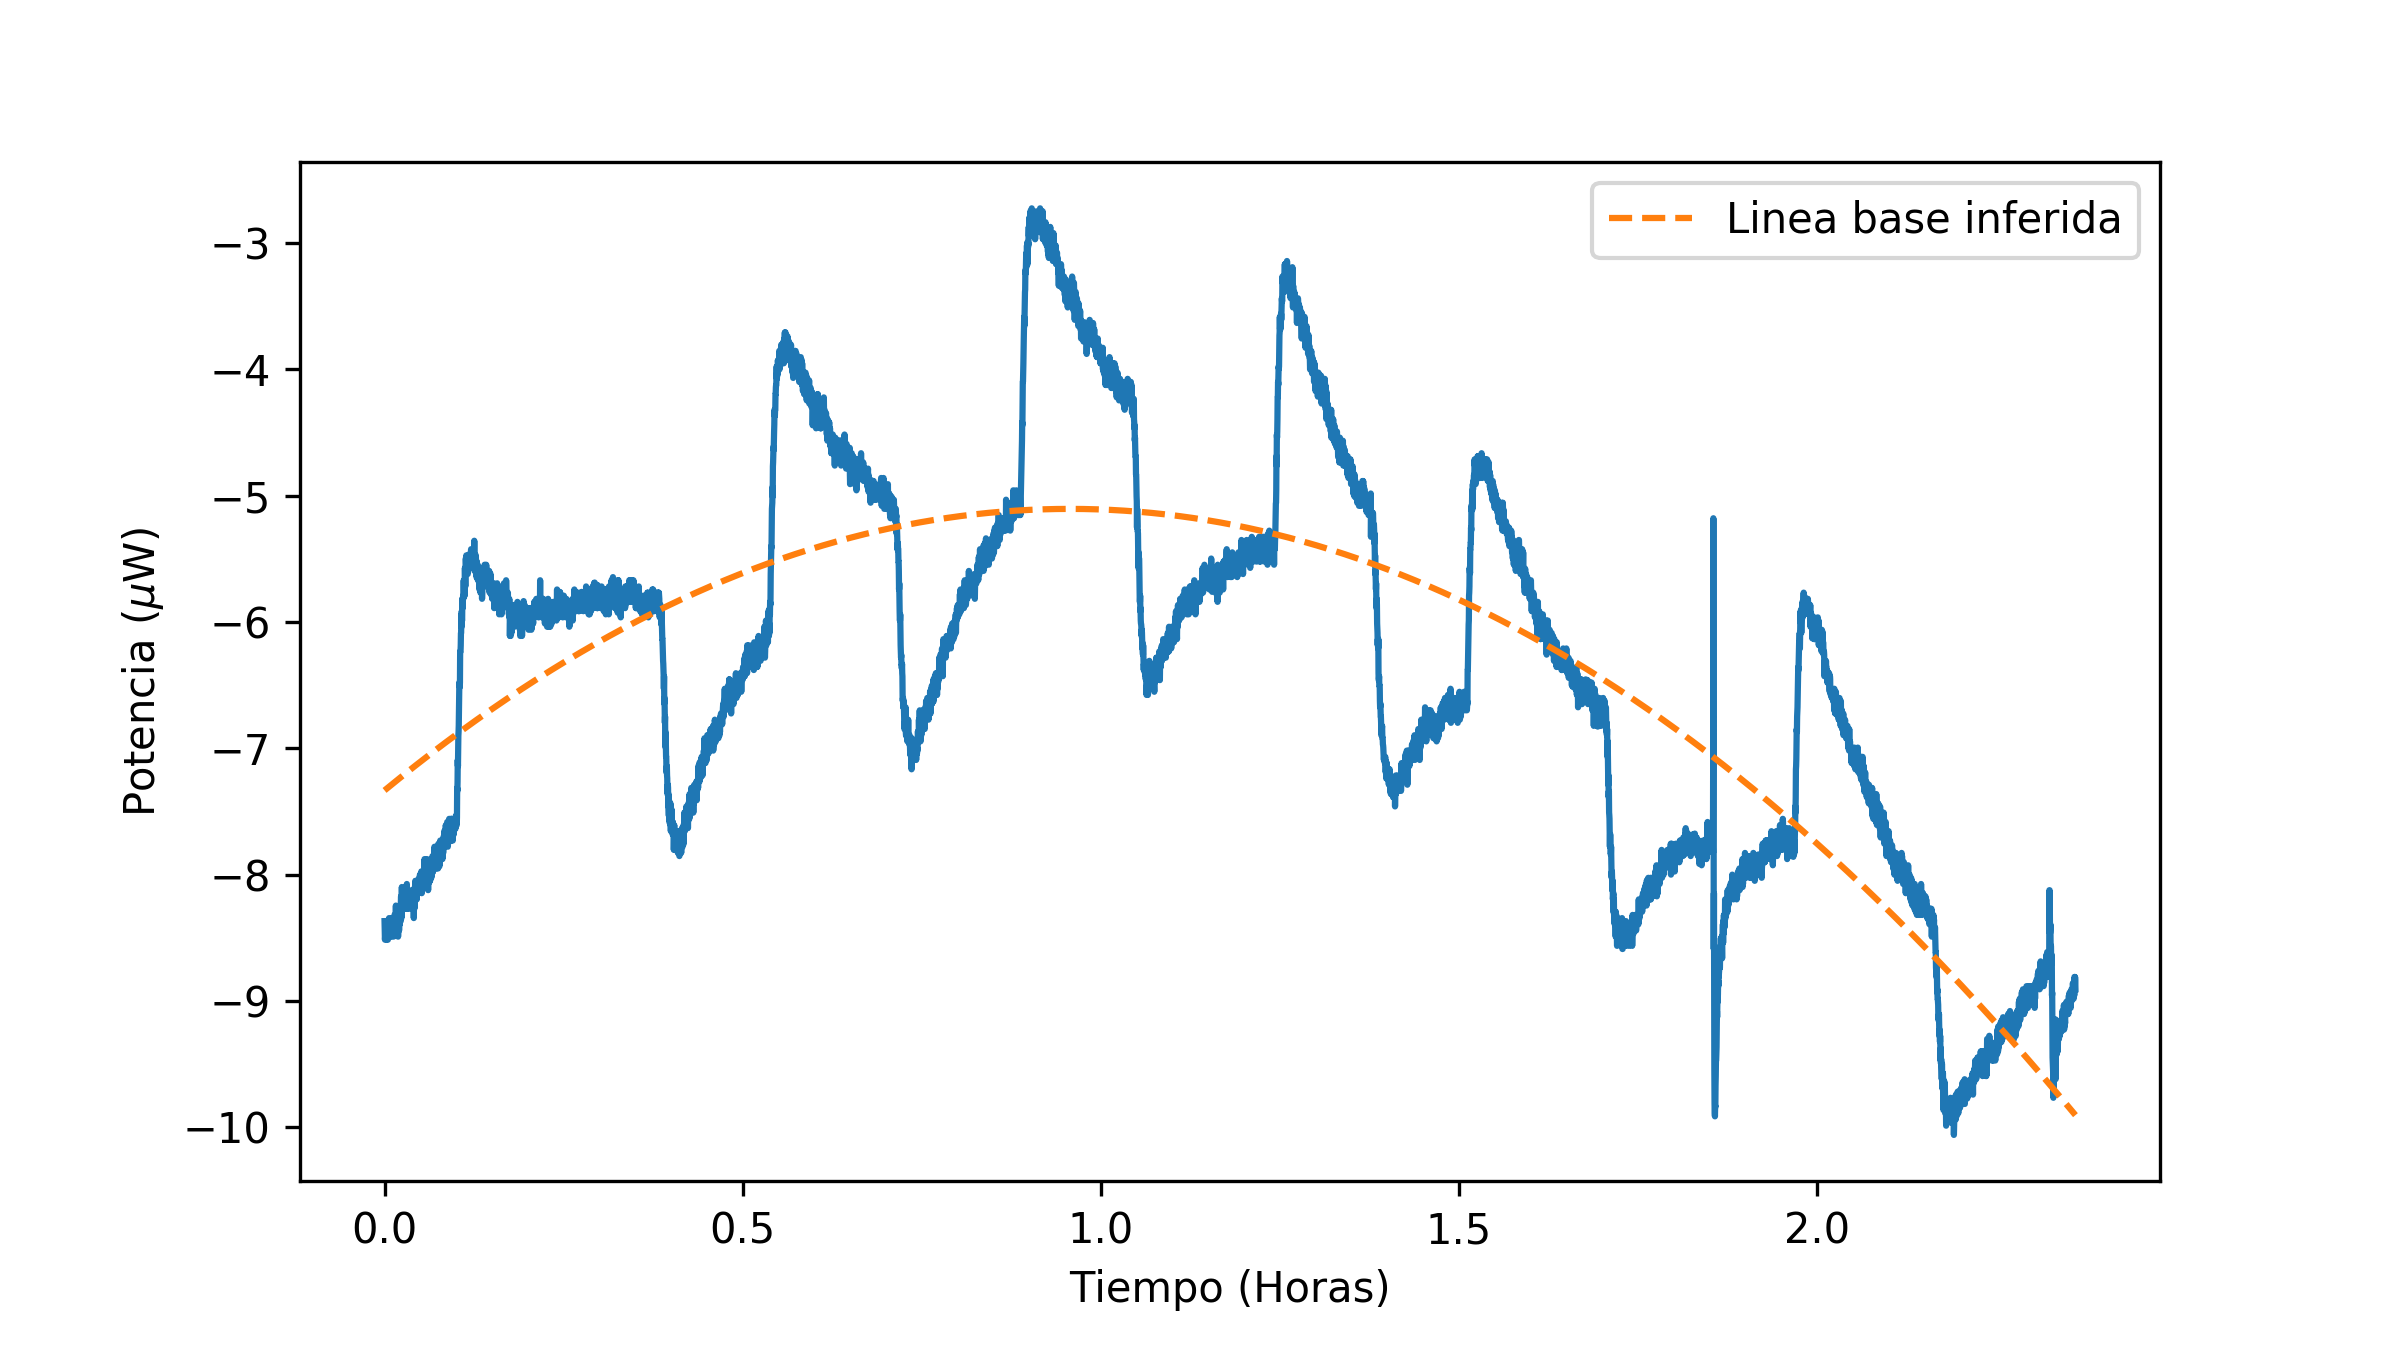
\includegraphics[width=\linewidth]{../Data/Baselines/motor}
		\caption{Las conexiones y desconexiones del agitador perturban la línea base, sin embargo, lentamente el equipo vuelve al equilibrio.}
		\label{fig: connection}
	\end{figure}
	


		